\section{Pruebas de bondad de ajuste}
\label{sec:3.9}

La \emph{prueba $\chi^{2}$} se usa comúnmente para comparar \emph{datos observados vs datos esperados} suponiendo que los datos siguen ciertas hipótesis.


Debemos suponer cierta hipótesis, la cuál nuestros datos seguirán y calculamos los datos esperados de acuerdo a esa hipótesis.


Debemos ya tener los datos observados, y calcular la desviación entre estos y los esperados usando el estadístico definido en la siguiente fórmula:
\begin{align}
	\texttt{valor }\chi^{2}\texttt{:} g= \sum\dfrac{\left( O-E \right)^{2}}{E},
\end{align}
donde $O$ es el valor observado y $E$ el esperado, con la suma sobre todos los posibles datos.

\subsection{Aplicaciones del estadístico $\chi-$cuadrada}
La prueba de ji cuadrado se puede usar para hacer lo siguiente:
\begin{itemize}
	\item Mostrar una relación causal o independencia entre una variable de entrada y otra de salida.
	\item Verificar si los datos observados provienen de una fuente justa / imparcial.
	\item Comprobar si los datos son demasiado buenos para ser verdad.
\end{itemize}


\subsection{Ejemplo}
Realicemos un experimento hipotético en el que una moneda se lanza 10 veces. ¿Cuántas veces espera obtener ya sea un reverso o un sol?  La respuesta adecuada sería 5.  Ahora bien, ¿qué pasaría si realizamos este experimento 1000 veces y registramos los números de reversos y soles.


Supongamos que observamos soles 553 veces y reversos el resto de ocasiones:
\begin{center}
	$H_{0}:$ La proporción de soles y reversos es $0.5$ \\
	$H_{a}:$ La proporción no es $0.5$
\end{center}



\begin{center}
	\begin{tabular}{|l|l|l|}\hline
		& Soles & reversos\\\hline
		Observado & 553 & 447\\\hline
		Esperado & 500 & 500\\\hline
	\end{tabular}
\end{center}


Calculemos el valor $\chi^{2}:$
\begin{align}
	g = \dfrac{\left( \left( 553-500 \right)^{2}+\left( 447-500 \right)^{2} \right)}{500}\approx 11.236
\end{align}



Este valor$-\chi^{2}$ se compara al valor en una \emph{distribución $\chi^{2}$} para un número dado de \emph{grados de libertad} y un nivel de significación.

\subsection{La Distribución $\chi^{2}$}
Sean $X_{1},X_{2},...,X_{\nu}$ variables aleatorias independientes $N(0,1).$
Consideremos la variable aleatoria
\begin{align}
	\label{outline:19}
	\chi^{2}=X_{1}^{2}+...+X_{\nu}^{2}
\end{align}
a la que llamaremos \emph{chi cuadrada.} Su correspondiente distribución de probabilidad recibe el mismo nombre.

\subsection{Propiedades de $\chi^{2}$}
\begin{align}
	\label{eq:3.9.1}
	\mu=\nu, \; \s = 2\nu
\end{align}


\lstinputlisting[language=Python]{../code/chi-cuadrada/statsChi2Simple.py}



\begin{figure}
	\centering
	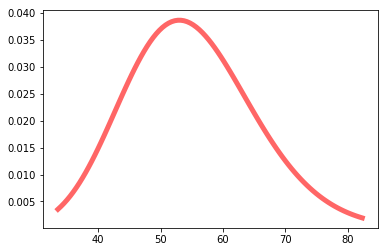
\includegraphics[height=5cm,keepaspectratio=true]{./images/statsChi2.png}
	% statsChi2.png: 0x0 pixel, 300dpi, 0.00x0.00 cm, bb=
	\caption{Función de densidad de distribución $\chi^2$ con $\nu=55$}
	\label{fig:3.9.1}
\end{figure}


\lstinputlisting[language=Python]{../code/chi-cuadrada/statsChi2.py}



\begin{center}
	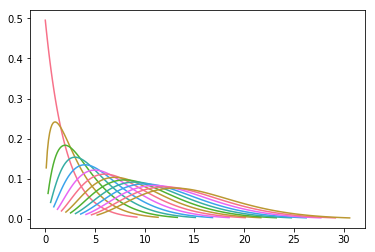
\includegraphics[height=7cm,keepaspectratio=true]{./images/statsChi2Several.png}
	% statsChi2Several.png: 0x0 pixel, 300dpi, 0.00x0.00 cm, bb=
\end{center}


\subsection{Prueba formal de bondad de ajuste}

\begin{teorema}[Prueba $\chi^2$ de bondad de ajuste]
	Sea una muestra clasificada en $k$ categorías mutuamente excluyentes con frecuencias observadas $O_1,\ldots,O_k$ ($\sum_i O_i = N$), y sea $H_0$ la hipótesis de que la población sigue una distribución teórica que asigna probabilidades $p_1,\ldots,p_k$ a dichas categorías. Bajo $H_0$, el estadístico
	\begin{align}
		\chi^2 = \sum_{i=1}^k \frac{(O_i-E_i)^2}{E_i}, \qquad E_i = Np_i,
	\end{align}
	se distribuye asintóticamente como $\chi^2_{\nu}$ con $\nu = k-1-m$ grados de libertad, donde $m\ge 0$ es el número de parámetros del modelo teórico que fueron estimados a partir de la misma muestra (si las probabilidades $p_i$ son completamente conocidas de antemano, $m=0$ y $\nu=k-1$).
\end{teorema}

\begin{observacion}[Regla de Cochran]
	La aproximación $\chi^2$ solo es confiable cuando las frecuencias esperadas no son demasiado pequeñas. La regla práctica de Cochran exige que ninguna $E_i$ sea menor a $1$, y que no más del $20\%$ de las celdas tengan $E_i<5$. Cuando esta condición se viola, la solución estándar es \emph{colapsar o fusionar} categorías adyacentes de baja frecuencia esperada hasta cumplirla, reduciendo correspondientemente los grados de libertad.
\end{observacion}

